\documentclass{standalone}
\usepackage{tikz}
\usetikzlibrary{patterns, positioning}


\begin{document}
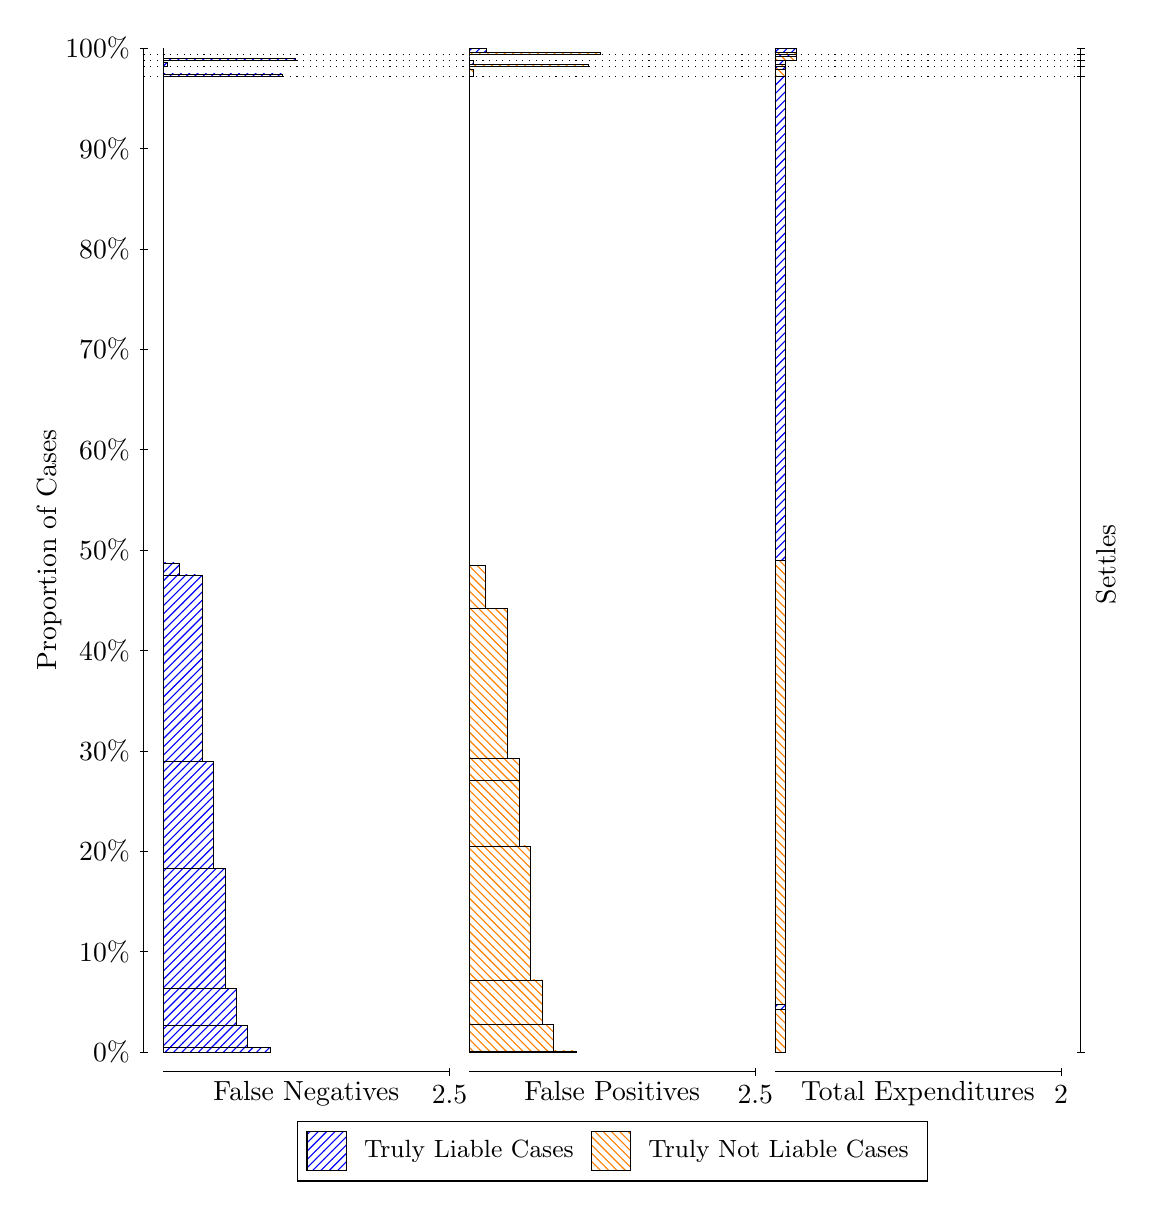
\begin{tikzpicture}
\draw[black, very thin] (1.5,1.75) -- (1.5,14.5);
\node[rotate=90, text=black, anchor=center] at (0.3, 8.125) {Proportion of Cases};
\draw[black, very thin] (1.45,1.75) -- (1.55,1.75);
\node[text=black, anchor=east] at (1.45, 1.75) {0\%};
\draw[black, very thin] (1.45,3.025) -- (1.55,3.025);
\node[text=black, anchor=east] at (1.45, 3.025) {10\%};
\draw[black, very thin] (1.45,4.3) -- (1.55,4.3);
\node[text=black, anchor=east] at (1.45, 4.3) {20\%};
\draw[black, very thin] (1.45,5.575) -- (1.55,5.575);
\node[text=black, anchor=east] at (1.45, 5.575) {30\%};
\draw[black, very thin] (1.45,6.85) -- (1.55,6.85);
\node[text=black, anchor=east] at (1.45, 6.85) {40\%};
\draw[black, very thin] (1.45,8.125) -- (1.55,8.125);
\node[text=black, anchor=east] at (1.45, 8.125) {50\%};
\draw[black, very thin] (1.45,9.4) -- (1.55,9.4);
\node[text=black, anchor=east] at (1.45, 9.4) {60\%};
\draw[black, very thin] (1.45,10.675) -- (1.55,10.675);
\node[text=black, anchor=east] at (1.45, 10.675) {70\%};
\draw[black, very thin] (1.45,11.95) -- (1.55,11.95);
\node[text=black, anchor=east] at (1.45, 11.95) {80\%};
\draw[black, very thin] (1.45,13.225) -- (1.55,13.225);
\node[text=black, anchor=east] at (1.45, 13.225) {90\%};
\draw[black, very thin] (1.45,14.5) -- (1.55,14.5);
\node[text=black, anchor=east] at (1.45, 14.5) {100\%};

\draw[black, very thin] (13.4,1.75) -- (13.4,14.5);
\draw[black, very thin] (13.35,1.75) -- (13.45,1.75);
\node[anchor=west] at (13.35, 1.75) {};
\draw[black, very thin] (13.35,14.14) -- (13.45,14.14);
\node[anchor=west] at (13.35, 14.14) {};
\draw[black, very thin] (13.35,14.266) -- (13.45,14.266);
\node[anchor=west] at (13.35, 14.266) {};
\draw[black, very thin] (13.35,14.343) -- (13.45,14.343);
\node[anchor=west] at (13.35, 14.343) {};
\draw[black, very thin] (13.35,14.422) -- (13.45,14.422);
\node[anchor=west] at (13.35, 14.422) {};
\draw[black, very thin] (13.35,14.5) -- (13.45,14.5);
\node[anchor=west] at (13.35, 14.5) {};

\draw[black, very thin, pattern color=blue, pattern=north east lines] (1.75,1.75) rectangle (3.1125,1.8107);
\draw[black, very thin, pattern color=blue, pattern=north east lines] (1.75,1.8107) rectangle (2.8218,2.0873);
\draw[black, very thin, pattern color=blue, pattern=north east lines] (1.75,2.0873) rectangle (2.6765,2.5541);
\draw[black, very thin, pattern color=blue, pattern=north east lines] (1.75,2.5541) rectangle (2.5312,4.08);
\draw[black, very thin, pattern color=blue, pattern=north east lines] (1.75,4.08) rectangle (2.3858,5.4371);
\draw[black, very thin, pattern color=blue, pattern=north east lines] (1.75,5.4371) rectangle (2.2405,7.8091);
\draw[black, very thin, pattern color=blue, pattern=north east lines] (1.75,7.8091) rectangle (1.9498,7.9603);
\draw[black, very thin, pattern color=orange, pattern=north west lines] (1.75,7.9603) rectangle (1.75,14.14);
\draw[black, very thin, pattern color=blue, pattern=north east lines] (1.75,14.14) rectangle (3.2578,14.172);
\draw[black, very thin, pattern color=orange, pattern=north west lines] (1.75,14.172) rectangle (1.75,14.266);
\draw[black, very thin, pattern color=blue, pattern=north east lines] (1.75,14.266) rectangle (1.8045,14.32);
\draw[black, very thin, pattern color=orange, pattern=north west lines] (1.75,14.32) rectangle (1.75,14.343);
\draw[black, very thin, pattern color=blue, pattern=north east lines] (1.75,14.343) rectangle (3.4213,14.37);
\draw[black, very thin, pattern color=orange, pattern=north west lines] (1.75,14.37) rectangle (1.75,14.422);
\draw[black, very thin, pattern color=orange, pattern=north west lines] (1.75,14.422) rectangle (1.75,14.448);
\draw[black, very thin, pattern color=blue, pattern=north east lines] (1.75,14.448) rectangle (1.75,14.5);
\draw[black, very thin, pattern color=orange, pattern=north west lines] (5.6333,1.75) rectangle (6.9958,1.7641);
\draw[black, very thin, pattern color=orange, pattern=north west lines] (5.6333,1.7641) rectangle (6.7052,2.1053);
\draw[black, very thin, pattern color=orange, pattern=north west lines] (5.6333,2.1053) rectangle (6.5598,2.6657);
\draw[black, very thin, pattern color=orange, pattern=north west lines] (5.6333,2.6657) rectangle (6.4145,4.3661);
\draw[black, very thin, pattern color=orange, pattern=north west lines] (5.6333,4.3661) rectangle (6.2692,5.1987);
\draw[black, very thin, pattern color=orange, pattern=north west lines] (5.6333,5.1987) rectangle (6.2692,5.4796);
\draw[black, very thin, pattern color=orange, pattern=north west lines] (5.6333,5.4796) rectangle (6.1238,7.3864);
\draw[black, very thin, pattern color=orange, pattern=north west lines] (5.6333,7.3864) rectangle (5.8332,7.9301);
\draw[black, very thin, pattern color=blue, pattern=north east lines] (5.6333,7.9301) rectangle (5.6333,14.14);
\draw[black, very thin, pattern color=orange, pattern=north west lines] (5.6333,14.14) rectangle (5.6878,14.234);
\draw[black, very thin, pattern color=blue, pattern=north east lines] (5.6333,14.234) rectangle (5.6333,14.266);
\draw[black, very thin, pattern color=orange, pattern=north west lines] (5.6333,14.266) rectangle (7.1412,14.288);
\draw[black, very thin, pattern color=blue, pattern=north east lines] (5.6333,14.288) rectangle (5.6878,14.343);
\draw[black, very thin, pattern color=orange, pattern=north west lines] (5.6333,14.343) rectangle (5.6333,14.395);
\draw[black, very thin, pattern color=blue, pattern=north east lines] (5.6333,14.395) rectangle (5.6333,14.422);
\draw[black, very thin, pattern color=orange, pattern=north west lines] (5.6333,14.422) rectangle (7.3047,14.448);
\draw[black, very thin, pattern color=blue, pattern=north east lines] (5.6333,14.448) rectangle (5.8513,14.5);
\draw[black, very thin, pattern color=orange, pattern=north west lines] (9.5167,1.75) rectangle (9.6529,2.2938);
\draw[black, very thin, pattern color=blue, pattern=north east lines] (9.5167,2.2938) rectangle (9.6529,2.3545);
\draw[black, very thin, pattern color=orange, pattern=north west lines] (9.5167,2.3545) rectangle (9.6529,7.9909);
\draw[black, very thin, pattern color=blue, pattern=north east lines] (9.5167,7.9909) rectangle (9.6529,14.14);
\draw[black, very thin, pattern color=orange, pattern=north west lines] (9.5167,14.14) rectangle (9.6529,14.234);
\draw[black, very thin, pattern color=blue, pattern=north east lines] (9.5167,14.234) rectangle (9.6529,14.266);
\draw[black, very thin, pattern color=orange, pattern=north west lines] (9.5167,14.266) rectangle (9.6529,14.288);
\draw[black, very thin, pattern color=blue, pattern=north east lines] (9.5167,14.288) rectangle (9.6529,14.343);
\draw[black, very thin, pattern color=orange, pattern=north west lines] (9.5167,14.343) rectangle (9.7892,14.395);
\draw[black, very thin, pattern color=blue, pattern=north east lines] (9.5167,14.395) rectangle (9.7892,14.422);
\draw[black, very thin, pattern color=orange, pattern=north west lines] (9.5167,14.422) rectangle (9.7892,14.448);
\draw[black, very thin, pattern color=blue, pattern=north east lines] (9.5167,14.448) rectangle (9.7892,14.5);
\draw[black, dotted] (1.5,14.14) -- (13.4,14.14);
\draw[black, dotted] (1.5,14.266) -- (13.4,14.266);
\draw[black, dotted] (1.5,14.343) -- (13.4,14.343);
\draw[black, dotted] (1.5,14.422) -- (13.4,14.422);
\draw[black, very thin] (1.75,1.5) -- (5.3833,1.5);
\node[text=black, anchor=north] at (3.5667, 1.5) {False Negatives};
\draw[black, very thin] (5.3833,1.45) -- (5.3833,1.55);
\node[text=black, anchor=north] at (5.3833, 1.45) {2.5};

\draw[black, very thin] (5.6333,1.5) -- (9.2667,1.5);
\node[text=black, anchor=north] at (7.45, 1.5) {False Positives};
\draw[black, very thin] (9.2667,1.45) -- (9.2667,1.55);
\node[text=black, anchor=north] at (9.2667, 1.45) {2.5};

\draw[black, very thin] (9.5167,1.5) -- (13.15,1.5);
\node[text=black, anchor=north] at (11.333, 1.5) {Total Expenditures};
\draw[black, very thin] (13.15,1.45) -- (13.15,1.55);
\node[text=black, anchor=north] at (13.15, 1.45) {2};

\node[text=black, centered, rotate=90] at (13.72, 7.9452) {Settles};





\draw (7.449999999999999,1.5) node[draw=none] (baseCoordinate) {};
\begin{scope}[align=center]
        \matrix[scale=0.5, draw=black, below=0.5cm of baseCoordinate, nodes={draw}, column sep=0.1cm]{
            \node[rectangle, draw, minimum width=0.5cm, minimum height=0.5cm, pattern color=blue, pattern=north east lines] {}; &
            \node[draw=none, font=\small, text=black] (B) {Truly Liable Cases}; &
            \node[rectangle, draw, minimum width=0.5cm, minimum height=0.5cm, pattern color=orange, pattern=north west lines] {}; &
            \node[draw=none, font=\small, text=black] (B) {Truly Not Liable Cases}; \\
            };
\end{scope}

\end{tikzpicture}
\end{document}